%!TEX root = ../template.tex
%%%%%%%%%%%%%%%%%%%%%%%%%%%%%%%%%%%%%%%%%%%%%%%%%%%%%%%%%%%%%%%%%%%%
%% chapter4.tex
%% NOVA thesis document file
%%
%% Chapter with lots of dummy text
%%%%%%%%%%%%%%%%%%%%%%%%%%%%%%%%%%%%%%%%%%%%%%%%%%%%%%%%%%%%%%%%%%%%

\typeout{NT FILE chapter4.tex}%

\chapter{Data Description and Management}
\label{cha:data}

Explain our sources of data to explore the methods developed in this work. Show why you chose this type of data and which purpose it has been used. 

The data used in this work focused mainly in the usage of biosignals that can be associated with an occupational scenario. This is to provide strong evidence that the methods developed, although applicable to any kind of time series, can be used for occupational health data. From public databases we used \gls{ecg}, \gls{abp}, \gls{emg}, \gls{acc} and \gls{gyro}. It is important to mention that for the sake of performance evaluation and comparison, several benchmark databases were used with a broad type of time series.

\section{Public Datasets}

\subsection{Classification Benchmark - UCR}

The University California Riverside (UCR) Time Series Archive was introduced in 2002 
and is one of the most used benchmarks for time series data mining tasks, specially for classification.  The datasets are diverse in terms of data type, data domain, difficulty, number of classes and dimensionality\cite{ucr}.
\par
Several \textit{python} distributions make it available to download. In this thesis, all UCR archive datasets from the \textit{pyts} distribution were used for classification tasks. These represent 107 datasets from 18 different data types (audio, devices, \gls{ecg}, \gls{eog}, \gls{eeg}, \gls{har}, etc...), which also are from many different domains, such as medical, financial, motion, entomology, etc...\cite{ucr}
\par
The list of datasets can be found on the following link \cite{ucr_site}.
 

\subsection{UCI Machine Learning Repository}

The University California Irvine (UCI) Machine Learning is another well known benchmark for machine learning tasks. It does not focus solely on time series data mining, having datasets for time series, image, text or categorical data. This archive was created as an ftp in 1987 by a studen at UC Irvine, containing now 607 datasets. 
\par
From this dataset, we focused in time series data for the validation of the proposed methods. More specifically, this dataset contains time series that can be used to validate the proposed novelty and cyclic segmentation. We mostly used multidimensional time series related with human activity recognition tasks.
\par
The following datasets were used:
\begin{itemize}
\item \textbf{Dataset 2 - Smartphone Dataset for Human Activity Recognition in Ambient Assisted Living} This dataset was gathered from an experiment on 30 volunteers. Each subject was wearing a smartphone on the waist while performing several activities: \textit{(1) Walking, (2) Walking Upstairs, (3) Walking Downstairs, (4) Sitting, (5) Standing and (6) Laying}. The activities were performed for approximately 60 seconds. The device recorder the internal accelerometer (ACC) and gyroscope (GYR) data at a constant rate of 50 Hz. Each activity has been categorized and labelled on the acquired data \cite{dataset2, dataset2_2}.\\
\textbf{Purpose:} This dataset was used in the context of change point detection, to test the method in estimating transitions between the performed activities from the accelerometer data.

\begin{figure}
\centering
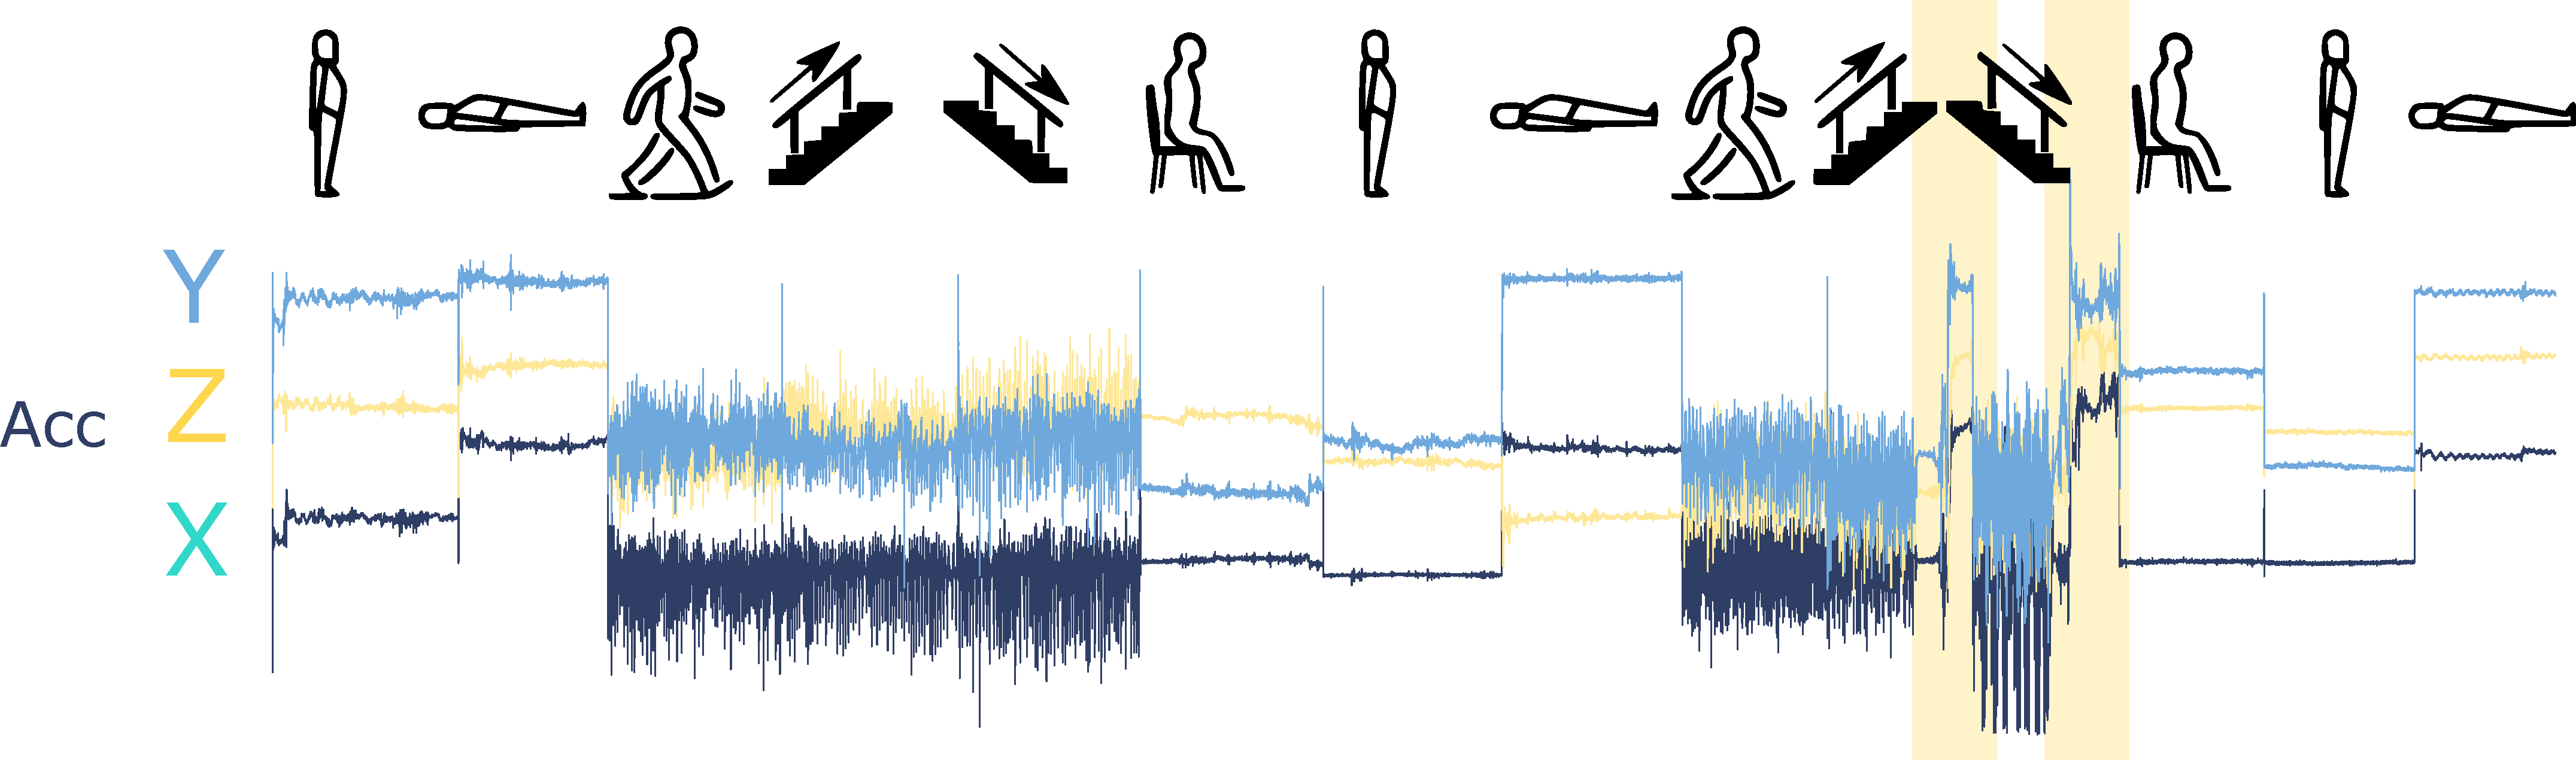
\includegraphics[width=\linewidth]{datasets/har_2_dataset.pdf}
\caption{•}
\label{fig:har2_dataset}
\end{figure}
    
\item \textbf{Dataset 3 - Smartphone Based Recognition of Human Activities and Postural Transitions}\\
The dataset was built in the context of human activity recognition experiments. These were carried out with a group of 30 volunteers that performed a protocol with six basic activities: three static postures (standing, sitting, lying) and three dynamic activities (walking, walking downstairs and walking upstairs). Additionally, the experiment also included postural transitions that occurred between the static postures. These are: stand-to-sit, sit-to-stand, sit-to-lie, lie-to-sit, stand-to-lie, and lie-to-stand. The data was collected with a smartphone (Samsung Galaxy S II) mounted on the waist of each subject. The data from a 3-axis accelerometer and 3-axis gyroscope was gathered at a constant rate of 50Hz. The experiments were video-recorded to label the data manually \cite{dataset3}.\\
\textbf{Purpose:} This dataset was used in the context of change point detection, to test the method in estimating transitions between the performed static and dynamic activities from the accelerometer and gyroscope data.

\begin{figure}
\centering
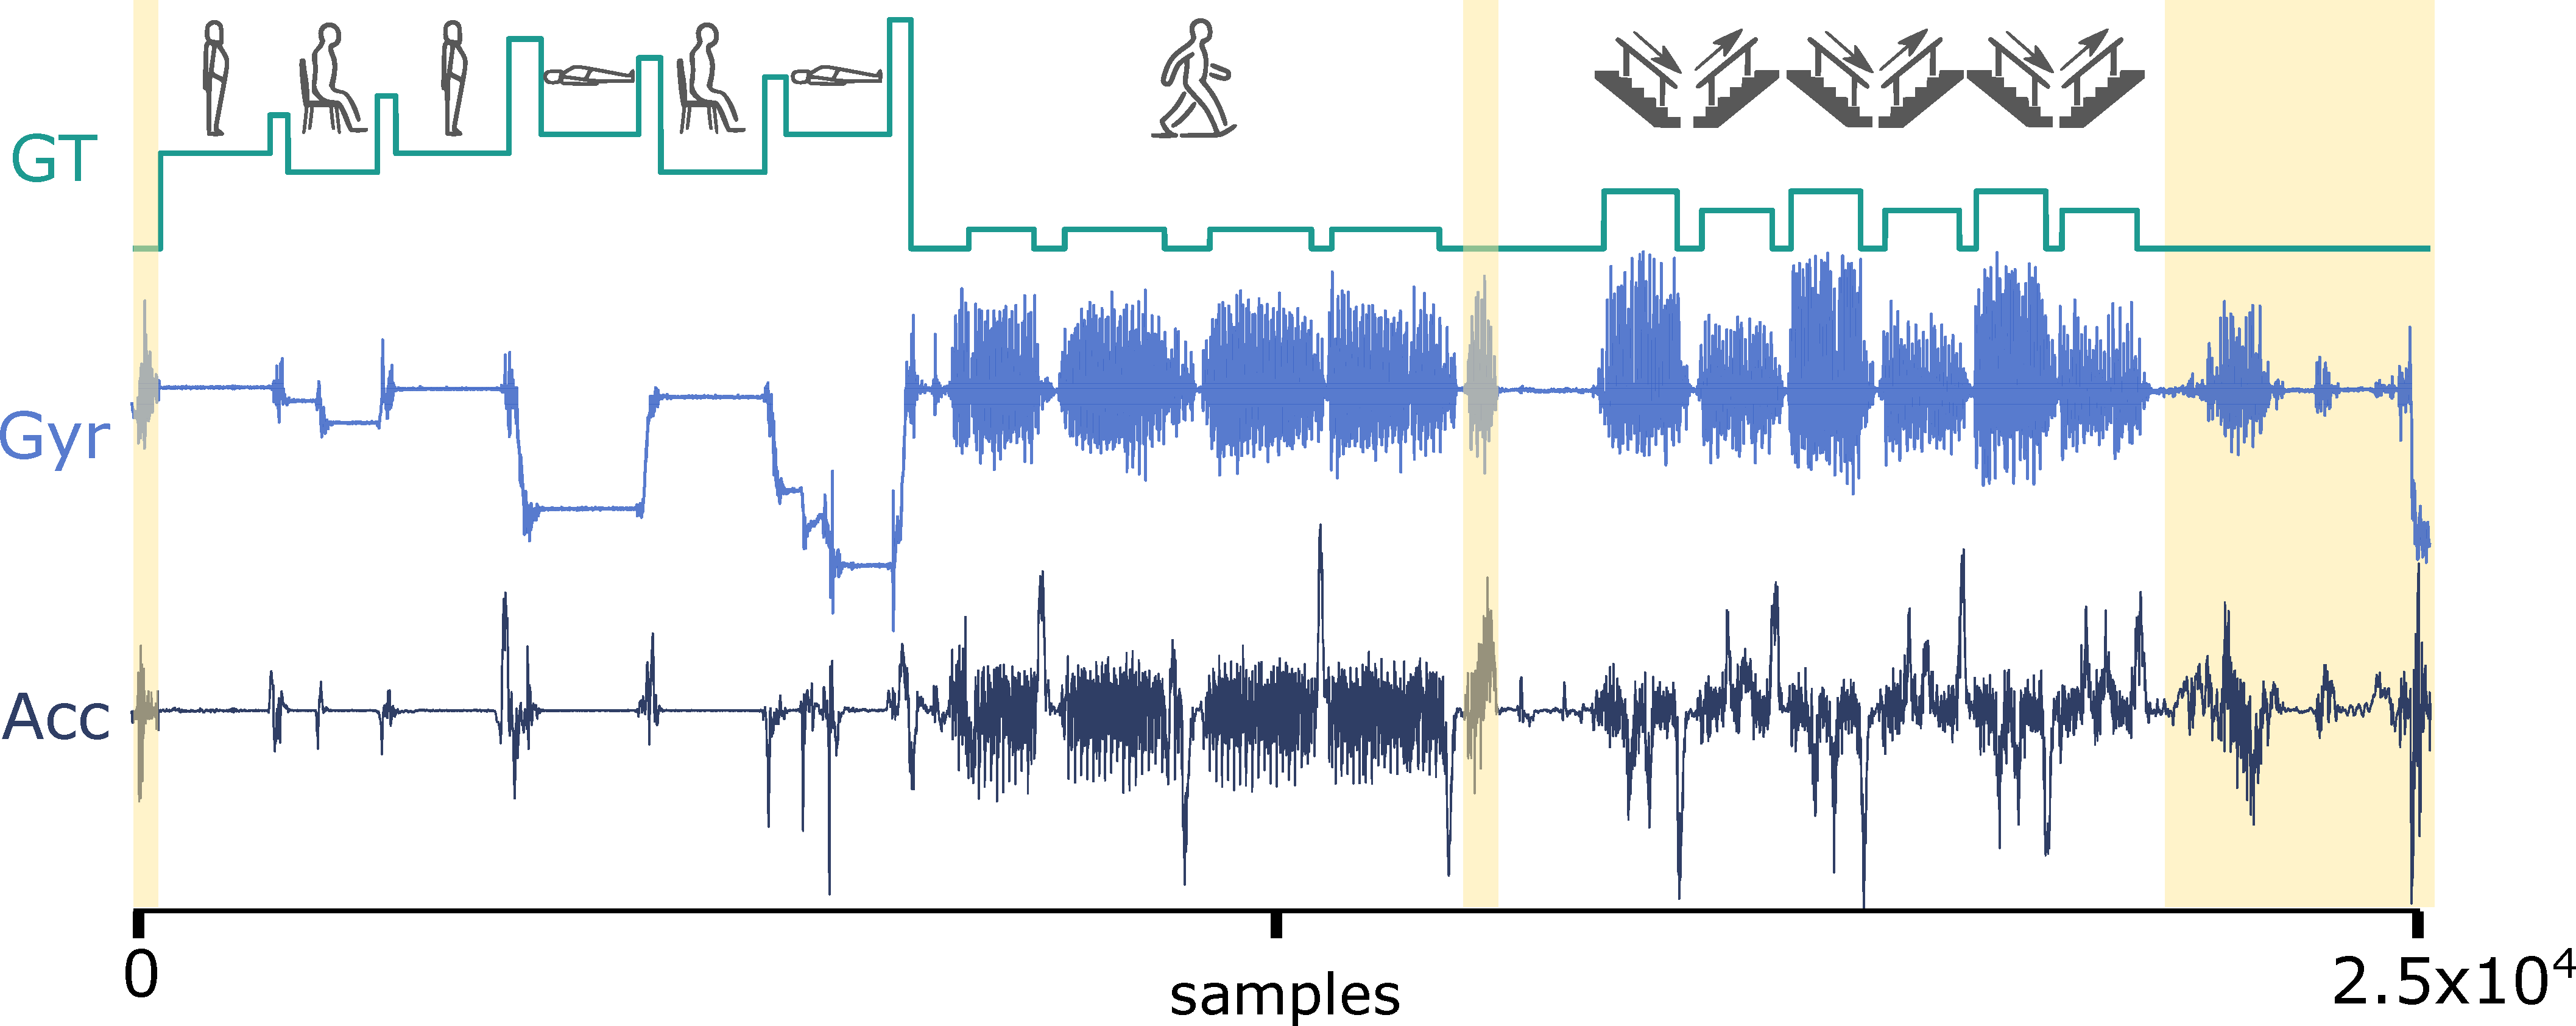
\includegraphics[width=\linewidth]{datasets/har_1_dataset.pdf}
\caption{•}
\label{fig:har1_dataset}
\end{figure}    
    
\item \textbf{Dataset 4 - Wireless Sensor Data Mining (WISDM) Smarphone and Smartwatch Activity Biometrics Dataset}\\
The raw data from the accelerometer and gyroscope sensors is collected from a smartphone and smartwatch at a rate of 20Hz. This experiment was conducted on 51 participants as they performed 18 activities, each for a duration of 3 minutes. Each sample of the data was labelled based on the activity it corresponds to. The activities are diverse and include dribbling, eating, jogging, sitting, walking on stairs, standing, walking, among others \cite{dataset4}.\\
\textbf{Purpose:} This dataset was used in the context of change point detection, to test the method in estimating transitions between the performed activities from the accelerometer and gyroscope data from both devices.

\begin{figure}
\centering
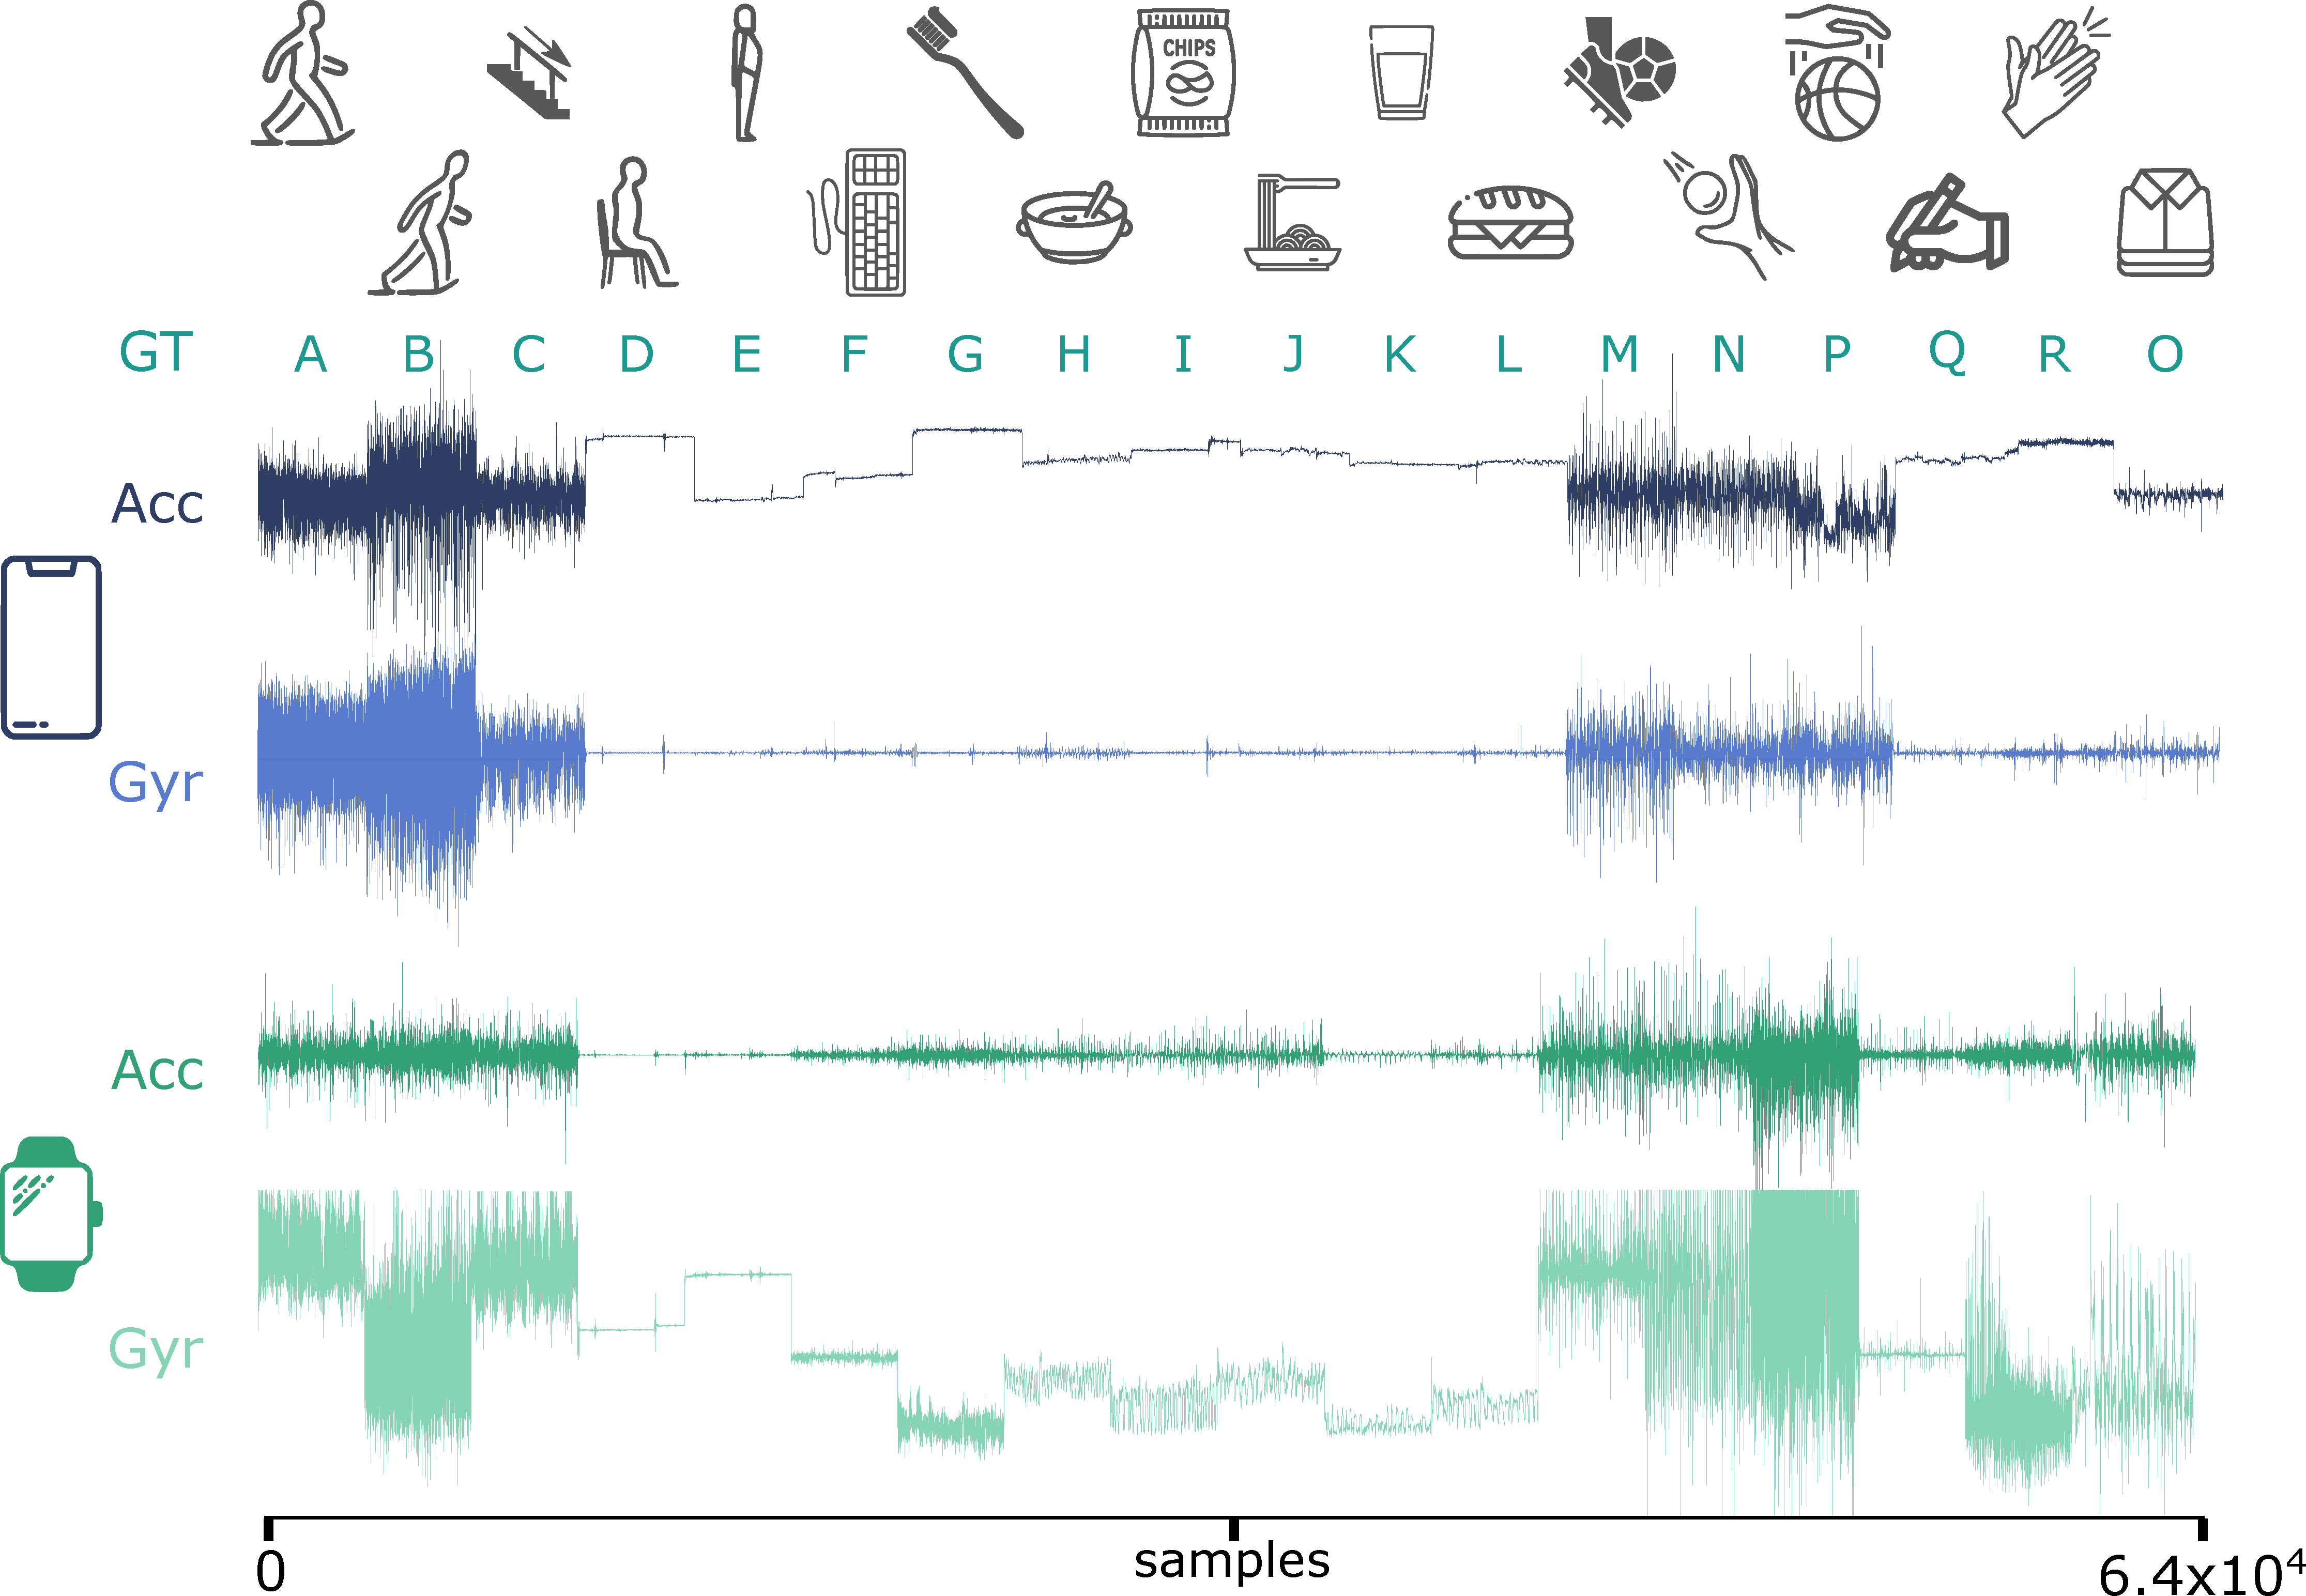
\includegraphics[width=\linewidth]{datasets/wisdim_dataset.pdf}
\caption{}
\label{fig:wisdim_data}
\end{figure}


    
\item \textbf{Dataset 5 - EMG Data for Gestures}\\
This dataset has EMG signals for recording patterns, by using a MYO Thalmic bracelet worn on a user's forearm. The bracelet is equipped with eight sensors equally spaced around the forearm that simultaneously acquire electromyographic signals. The dataset has raw EMG data from 36 subjects while they performed series of static hand gestures. The subject performs two series, each of which consists of six basic gestures. Each gesture was performed for 3 seconds with a pause of 3 seconds between gestures. The data was collected with a fixed sampling frequency of 200 Hz \cite{dataset5}.\\
\textbf{Purpose:} This dataset was used in the context of change point detection, to test the method in estimating transitions between the activation and relaxation of the muscular activity.

\begin{figure}
\centering
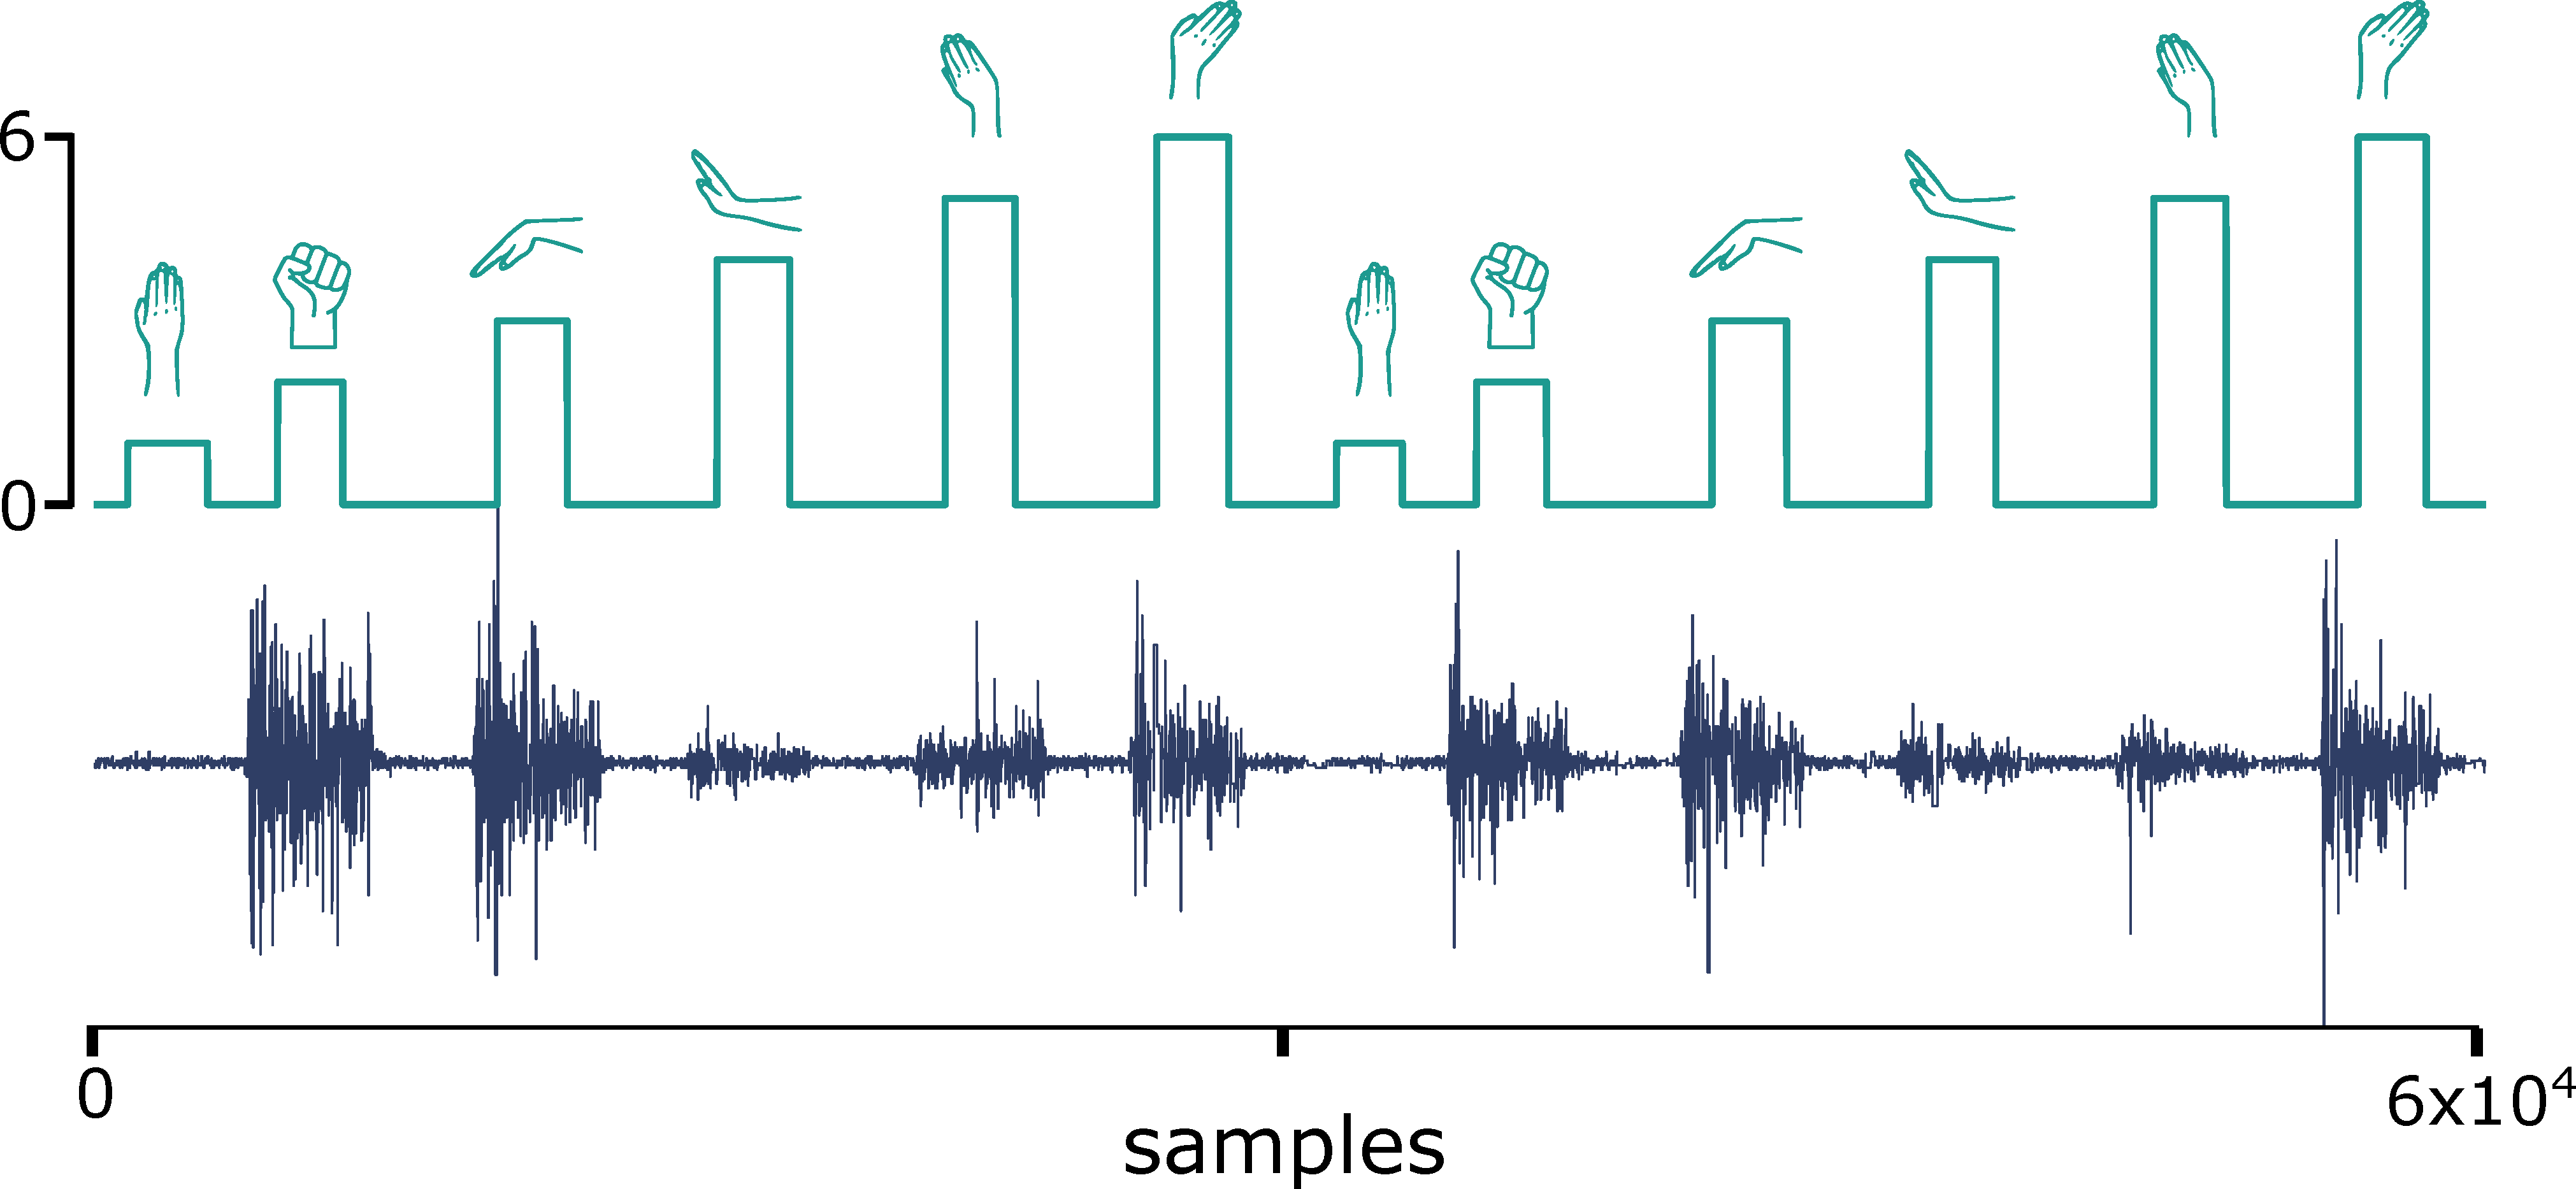
\includegraphics[width=\linewidth]{datasets/emg_dataset.pdf}
\caption{•}
\label{fig:emg_dataset}
\end{figure}


As indicated on Figure \ref{fig:emg_dataset}, the ground truth would have considered as events the absence of activity (which the original dataset uses because it was designed for a classification problem). In this case, we did not considered these events in our ground truth for this dataset.
    
    
    \item \textbf{Dataset 8 - } The dataset comprises several time series from real-world data. It was built from a project of the Alan Turing Insitute to have a repository for the evaluation of change point detection algorithms. The available benchmark page was used to get access to the datasets, and run the performance metrics developed. This way, the performance of the proposed method is compare with the performance of several existing methods \cite{cpd_alan}.
    \par
    \textbf{Purpose:} This dataset has ground-truth events for each time series. The performance of several existing methods is available and used to compare with the performance of the proposed method on the same time series.

\end{itemize}
    
\subsection{Kaggle}

\textbf{Dataset 1 - }\\
The dataset comprises data from 15 subjects that were performing 7 activities while wearing a sole wearable accelerometer mounted on the chest. The data was acquired at a constant rate of 52 Hz. The categories of activities are: \textit{(1) Working at computer, (2) Standing Up, Walking and Going Up/Down stairs, (3) Standing, (4) Walking, (5) Going Up/Down Stairs, (6) Walking and Talking with Someone, (7) Talking while Standing}. Each sample of the data gathered has a corresponding label from the performed activity \cite{dataset1}.\\

\textbf{Purpose:} This dataset was used in the context of novelty segmentation, to test the method in estimating transitions between the performed activities from the accelerometer data.

\subsection{Physionet}

\textbf{Dataset 6 - } The dataset comprehends 12 half-hour \gls{ecg} recordings and 3 half-hour recordings of noise typical in ambulatory \gls{ecg} recordings. The noise recordings were made using physically active volunteers and standard \gls{ecg} recorders, leads, and electrodes. The three noise records were assembled from the recordings by selecting intervals that contained predominantly baseline wander (in record 'bw'), muscle (EMG) artifact (in record 'ma'), and electrode motion artifact (in record 'em'). Two clean \gls{ecg} signals were selected and noise was added with different signal-to-noise ratios (SNR) \cite{dataset6, PhysioNet}.\\

\begin{figure}
\centering
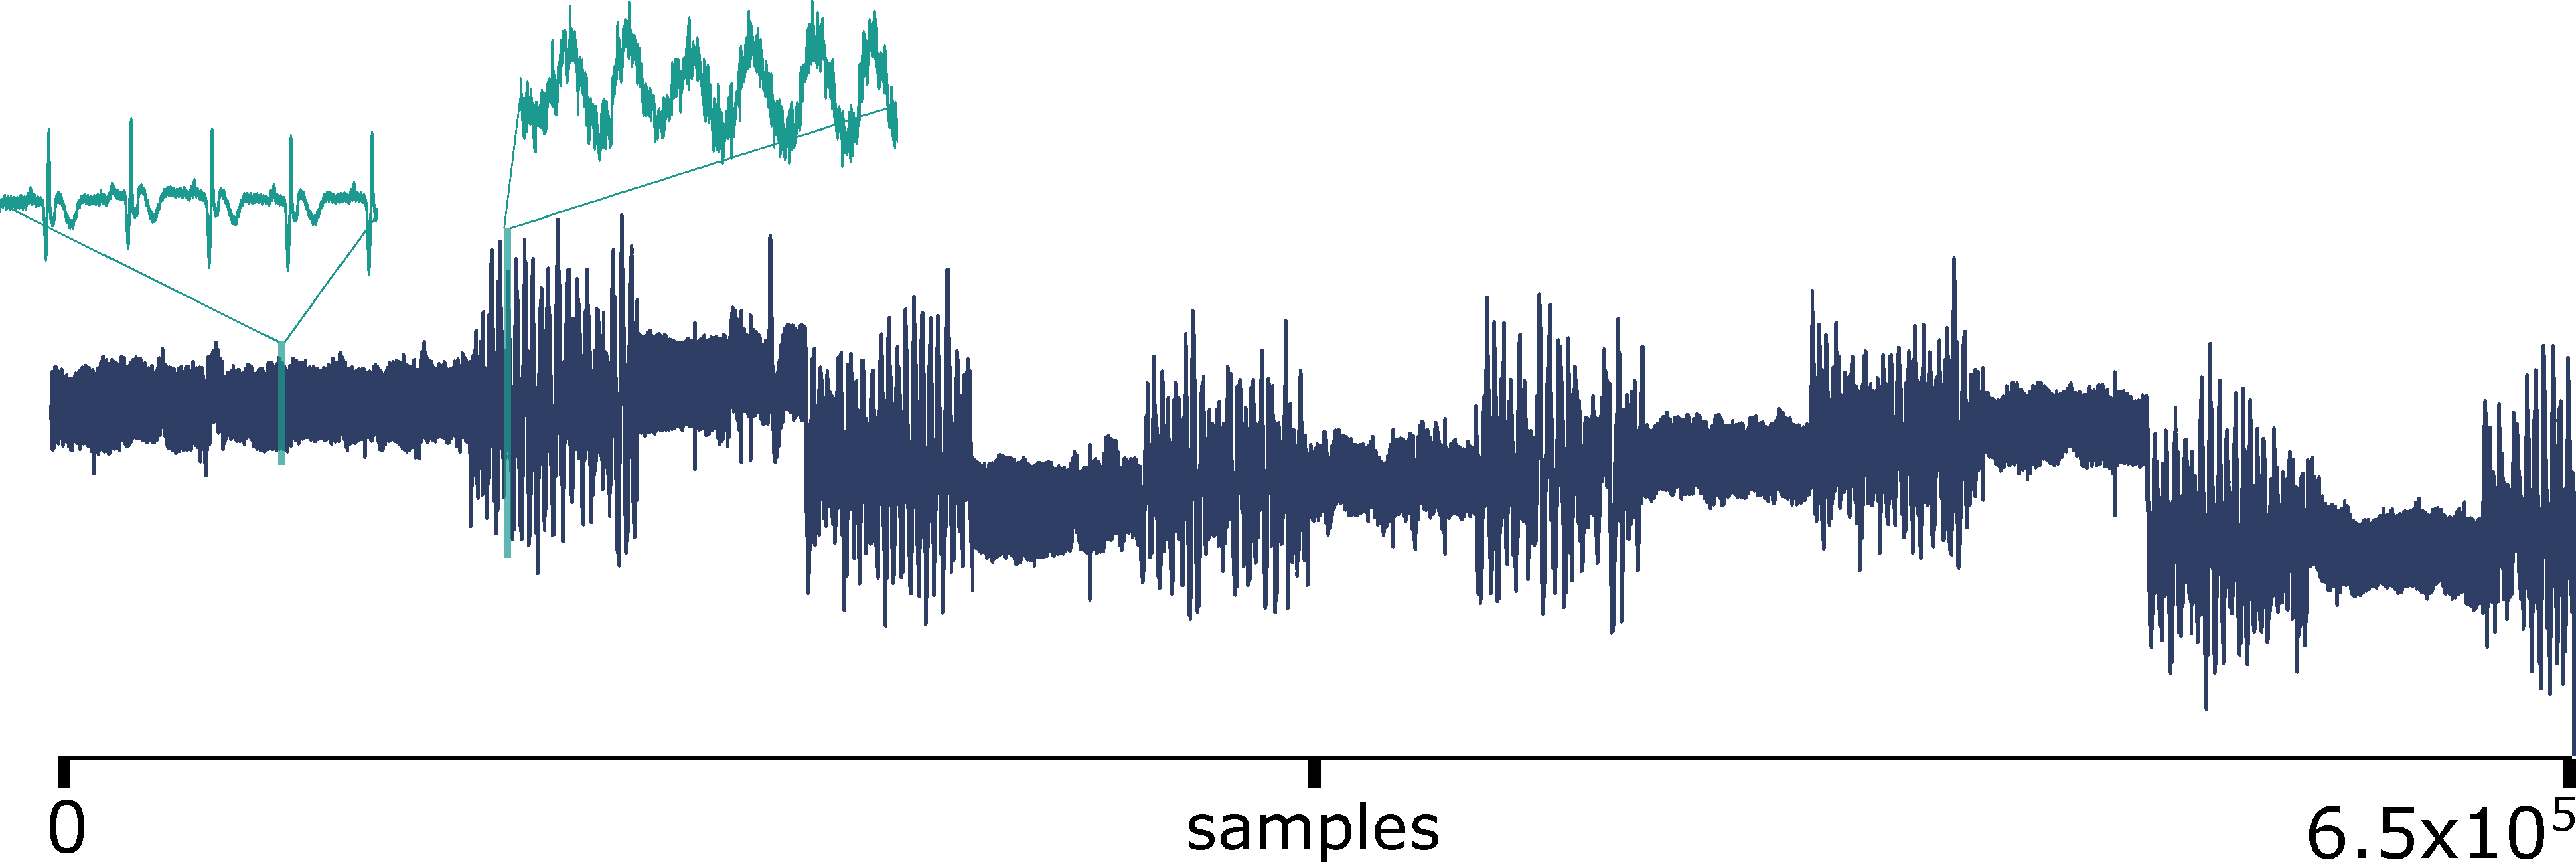
\includegraphics[width=\linewidth]{datasets/ecg_noise1.pdf}
\caption{•}
\label{fig:ecg1_dataset}
\end{figure}

\textbf{Purpose:} This dataset was used in the context of change point detection, to test the method in estimating transitions to and from noise sections of the signal.
    
\textbf{Dataset 7 - } This dataset has short duration \gls{ecg} signals, which were recorded from a healthy 25-year-old male performing different physical activities (standing, walking and single jump) to study the effect of motion artifacts on \gls{ecg} signals and their sparsity. The dataset was acquired with a sampling rate of 500 Hz and 16 bit resolution. For this exercise, only the records with jump were used \cite{dataset7, PhysioNet}.\\

\begin{figure}
\centering
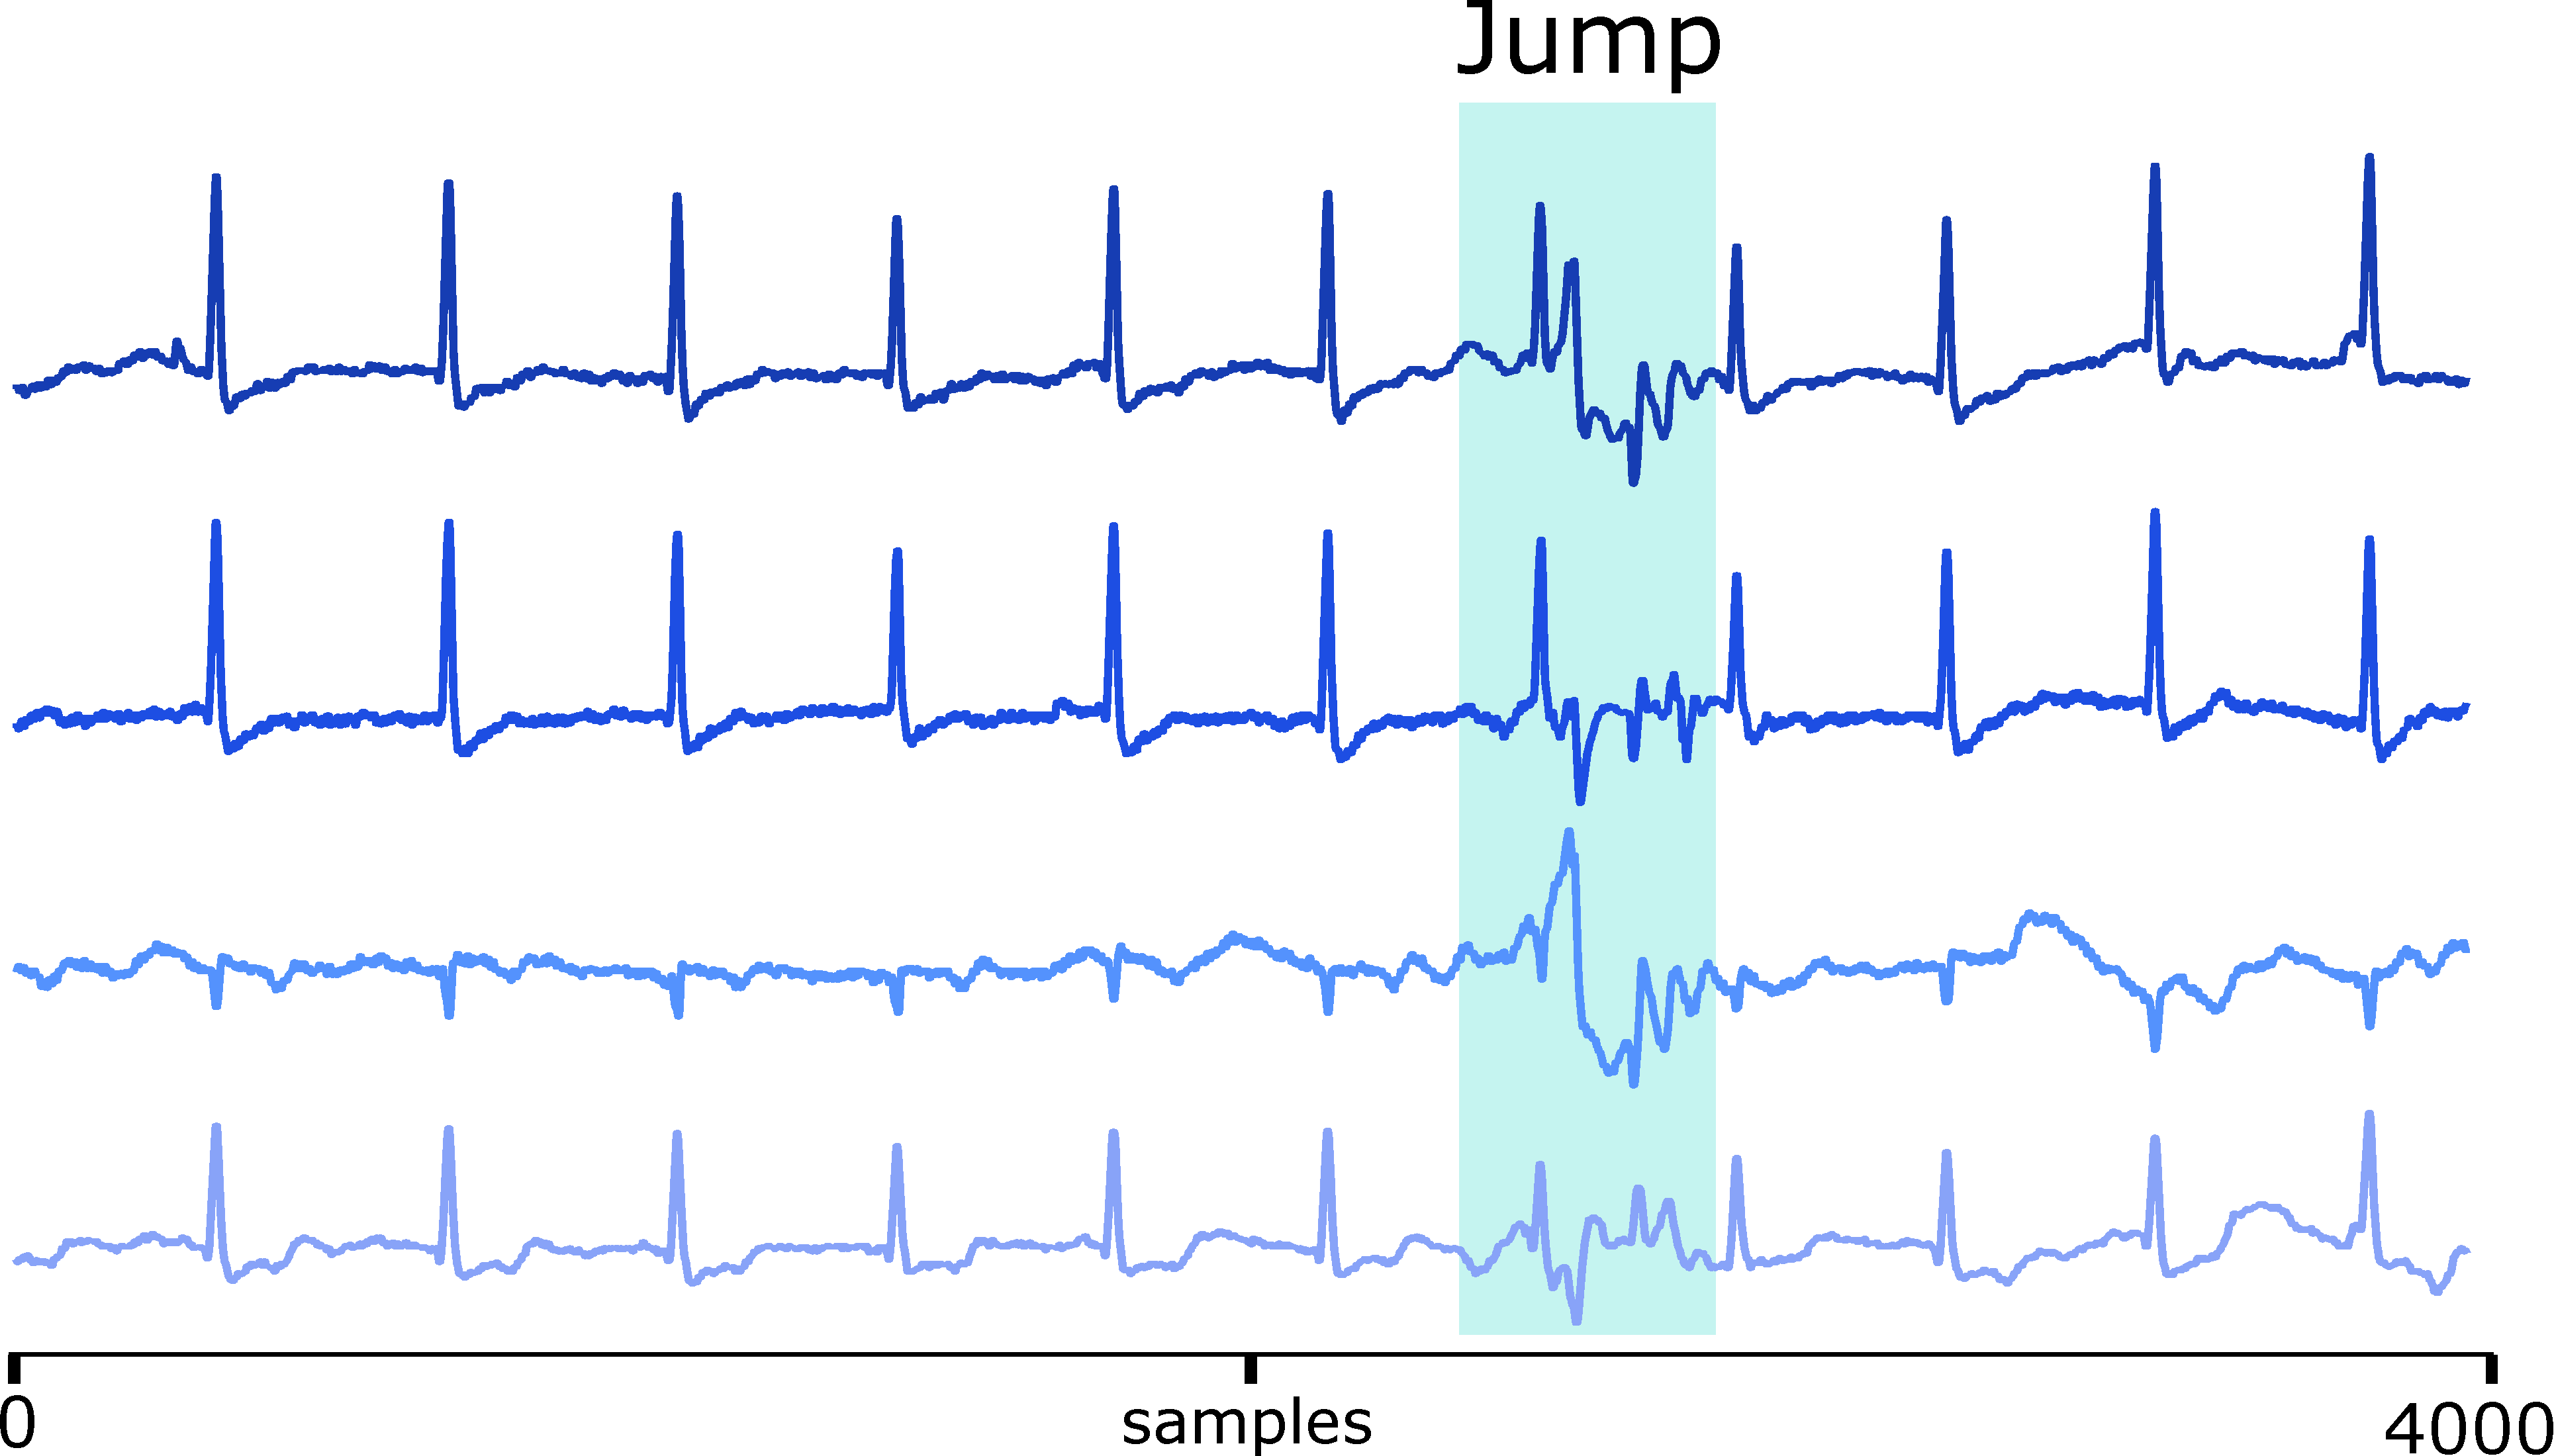
\includegraphics[width=\linewidth]{datasets/ecg_noise2.pdf}
\caption{•}
\label{fig:ecg2_dataset}
\end{figure}

\textbf{Purpose:} This dataset was used in the context of change point detection, to test the method in estimating transitions to and from noise sections of the signal.


\subsection{Alan Turing CPD Benchmark}
\label{sec:dataset8}

The Alan Turing Change Point Detection Benchmark is a recent dataset used to have a standard reference for change point segmentation tasks. The benchmark was created in 2020 and provides 42 datasets, being 42 univariate time series and 4 multi dimensional time series. It contains data from real scenarios that varies from finance, weather, society and medical:

\textbf{Dataset 8 - Alan Turing CPD Benchmark}\\
The dataset comprises several time series from real-world data. It was built from a project of the Alan Turing Insitute to have a repository for the evaluation of change point detection algorithms. The available benchmark page was used to get access to the datasets, and run the performance metrics developed. This way, the performance of the proposed method is compare with the performance of several existing methods \cite{cpd_alan}.\\

\textbf{Purpose:} This dataset has ground-truth events for each time series. The performance of several existing methods is available and used to compare with the performance of the proposed method on the same time series.

\section{Private Datasets}

\subsection{Aritrokinematic Dataset}

For this thesis, there were allowed access to inertial acquisitions made in the context of human activity recognition. The database used was obtained on the scope of the \textit{Arthrokinemat} project whose main objective was the development of a learning adaptive sensor-based measurement system to prevent osteoarthritis\cite{arthrokinemat}. More specifically, the recording was made for the work of \cite{Liu2019}, which introduces a human activity recognition system able to recognize between a list of several daily activities.
%intro

%contexto de aquisição
A set of multiple Biosensors were used, with various internal characteristics. Beginning with two \textit{8 channel PLUX hubs} a device which allows for the wireless acquisition of biosensors via Bluetooth, with them being part of the \textit{biosignals plux Research Kits}. From both \textit{plux hubs} there were used two 3-axial \gls{acc} sensors, 4 sets of \gls{emg} sensors and an electrogoniometer, with more details about these sensors being displayed in Table \ref{tab:plux_hubs}.

Adding to these sensors there were also used 4 other types of biosensors: one airborne microphone, one piezoelectric microphone, two 3-axial gyroscopes and one force sensor. From here, 18 activities were performed recursively, with all of these being listed in Table \ref{tab:hui_actvs}


\begin{table}[ht]
	\caption[\textit{Plux Hub} sensors descriptions, for the \gls{har} database]{\textit{Plux Hub} sensors descriptions, for the \gls{har} databases\cite{Liu2019}. The sensors are divided in half by a horizontal dash line with the first group of sensors using a single \textit{Plux Hub} device and the other sensors using the second device. The information provided by each sensor include also the positioning of the sensors as well as it's sampling frequency.}.
	\label{tab:plux_hubs}
\centering
\begin{tabular}{lll}
	\toprule
	\textbf{Sensor} & 
	\textbf{Position / Muscle} &
	\textbf{Sampling Frequency}\\
    \midrule
3 axial Upper Accelerometer & Thigh, proximal ventral & 100 Hz \\
3 axial Lower Accelerometer & Shank, distal ventral & 100 Hz \\
Eletrogoniometer & Knee of the right leg, lateral & 100 Hz \\
EMG1 & Musculus vastus medialis & 1000 Hz \\
EMG2 & Musculus tibialis anterior & 1000 Hz \\
EMG3 & Musculus biceps femoris & 1000 Hz \\
EMG4 & Musculus gastrocnemius & 1000 Hz \\
\bottomrule
\end{tabular}
\end{table}

\begin{table}[ht]
	\caption[Activities description, of the \gls{har} database]{Activities description, of the \gls{har} database\cite{Liu2019}. For each activity is displayed the number of repetitive occurrences each activity is performed as well as the total time length and the minimum and maximum length of each occurrence.}.
	\label{tab:hui_actvs}
\centering
\begin{tabular}{lllll}
	\toprule
	\textbf{Activity} & 
	\textbf{Occurrence} &
	\textbf{Total Length} & 
	\textbf{Min Length} &
	\textbf{Max Length}\\
    \midrule
 sit & 47 & 123.75s & 0.86s & 4.69s\\
 stand & 46 & 127.70s & 1.36s & 4.73s \\
 sit-to-stand & 45 & 30.94s & 0.15s & 1.30s\\
 stand-to-sit & 53 & 72.90s & 0.56s & 3.10s\\
 stair-up & 55 & 190.45s & 1.59s & 4.93s\\
 stair-down & 57 & 181.96s & 1.37s & 4.86s\\
 walk & 220 & 554.07s & 1.18s & 4.78s\\
 curve-left-step & 57 & 143.09s & 1.10 & 3.87s\\
 curve-left-spin & 46 & 109.15s & 1.25s & 3.39s\\
 curve-right-step & 51 & 67.51s & 0.54s & 3.19s \\
 curve-right-spin & 48 & 41.50s & 0.28s & 1.88s \\
 run & 97 & 151.27s & 0.64s & 2.74s\\
 v-cut-left & 53 & 43.76 & 0.29s & 2.08s\\
 v-cut-right & 55 & 61.75s & 0.35s & 2.37s\\
 lateral-shuffle-left & 53 & 97.54s & 0.73s & 4.11s \\
 lateral-shuffle-right & 52 & 90.42s & 0.75s & 3.98s\\
 jump-one-leg & 59 & 61.36s & 0.33s & 2.85s \\
 jump-two-leg & 63 & 63.40s & 0.51s & 1.63s\\
 \hline
 \textbf{Total} & \textbf{1157} & \textbf{2212.52s} & \textbf{0.15s} & \textbf{4.93s}\\
\bottomrule
\end{tabular}
\end{table}

The activities \textbf{sit-to-stand} and \textbf{stand-to-sit} were moments of transition between the activities stand and sit. Moreover the activities \textbf{curve-left} and \textbf{curve-right} were interposed between the activity of \textbf{walking}. \textbf{curve-left/right} are also divided into \textbf{step} or \textbf{spin}, depending if it is a big 90\degree turn with several walking steps or a fast 90\degree turn of the entire body like a parade command, respectively.

Another set of activities that may also require further explanation are \textbf{lateral-shuffle-left/right}, a motion usually done in sports that describes the subject's lateral movement of the left/right foot, with the other foot following along and continuing the shuffling in the same direction. \textbf{V-cut-left/right} means that the subject changes his direction by 90\degree at jogging speed. The remaining activities are self explanatory.

This database was used to study how the algorithm could be used to detect periodic events with different levels of motion cycle complexity. 

\subsection{Industrial Job Dataset}

This database has greater importance in comparison with the previous ones, as it will serve to test if this methodology is indeed valid for processing data acquired from a work environment. With this said, two main requirements need to be presented. Firstly, the data should have been retrieved in a real-working setting (i.e. not in a laboratory controlled environment), and secondly, it had to be the result of a direct sensor acquisition system that could provide information about the motion of the various workers.
%main requirements of the aquisition

The data acquisition was made in a previous thesis project from \cite{santos2019}, whose main objective was to calculate the ergonomic risk through  direct measuring data. 
The technological setting was provided by a sensing framework named Internet of Things in Package (IoTiP), designed and provided by Fraunhofer AICOS. IoTiP is a system that intends to combine hardware, firmware and software components to promote the field "Internet of Things"\cite{FraunhoferAICOS}. For this work, the technology setting consisted on 4 9-\gls{dof} \gls{imu} sensors (composed internally by a triaxial \gls{acc}, triaxial \gls{gyro} and triaxial \gls{mag}) and an Android wireless communication system. The last one was made through an application called Recorder, also developed by Fraunhofer AICOS.\cite{santos2019}.
%technology description
%tentei não entrar em muito detalhe visto que isto está na tese da Sara, tentei abordar os topicos todos dela mas da forma mais resumida possivel.


The acquisition was made in a Volkswagen Industrial assembly line where 12 manufacturing workers performed their work tasks while having attached 4 \gls{imu} sensors in their bodies.
%falar da interferencia dos sensors
During the acquisition, the subjects performed various tasks in multiple workstations. Relevantly to this thesis, the database comprehends three different workstations from \textit{Bodyshop assembly line}, a section where cars' doors were assembled: 1) Liftgate workstation, where back doors are mounted; 2) Fender workstation, involving front door tasks and 3) Doors workstation, which demanded tasks on the front doors and in the cars' hood\cite{santos2019}. The acquisitions made involved a total of 6 operators with each one performing at least 2 different workstations. The various acquisitions were simultaneously filmed and to synchronize the ground manual annotations of the data, in the beginning and end of the acquisition the subjects were asked to stay, firstly, in a neutral anatomic position and then perform a T pose (calibration position) as represented

% in Figure \ref{fig:t_pose}. 

There were also registered some details regarding the anthropomtetric characteristics of the various subjects, as displayed in Table. 

% \ref{tab:subj_char}.
%aquisition setting

The mentioned study was centered on the ergonomic assessment of the dominant arm. For this reason, the \gls{imu}s  were attached in: 1) the posterior side of the hand, 2) posterior side of the forearm and 3) posterior side of the arm and a final one 4) placed in the anterior side of the thorax area. All of the devices were attached with elastic bands, in such a way that all had their Y-axis pointed up while in a neutral anatomical position, as illustrated in Figure. 

% \ref{fig:imu_schem}. 

The last device is unique as in its original work it allowed an assessment of the movement of the arm in relation to the entire body. Moreover, it is also different from the other since its \gls{imu} sensor was incorporated in a smartphone. Smartphones can indeed work as \gls{imu} devices, since these can sense the acceleration, angular momentum and magnetic field.
% With this units being designated by IMU 1, IMU 2, IMU 3 and IMU 4, respectively.
Each one of these 4 \gls{imu} devices had incorporated within them 3 triaxial sensors (\gls{acc}, \gls{gyro}, \gls{mag}), with each producing a multivariate time series of 3 dimensions correspondent to the 3 coordinate orientations of x, y and z.

%\begin{figure}[ht]
%\begin{adjustwidth}{-1cm}{-1.2cm}
%\centering
%\begin{minipage}{.4\textwidth}
%    \includegraphics[width=1\linewidth]{Chapters/Figures/4_2_T pose.png}
%    \caption[T pose for synchronization]{T pose for synchronization of the various IMU devices.}
%    \label{fig:t_pose}
%\end{minipage}
%\begin{minipage}{.05\textwidth}
%\hspace*{0.5cm}\\
%\end{minipage}
%\begin{minipage}{.5\textwidth}
%    \includegraphics[width=1.1\linewidth]{Chapters/Figures/4_1_IMU placement squematic.pdf}
%    \caption[Schematic placements of IMU sensors]{Schematic placements of IMU sensors over the acquisition of \textit{Industrial} Database.}
%    \label{fig:imu_schem}
%\end{minipage}
%\end{adjustwidth}
%\end{figure}

The data is hierarchically divided, as showed in 
% \ref{fig:db_schem}. 

The Database is firstly divided into 12 groups corresponding to 6 subjects with each working at two different workstations; followed by 4 other databases: Hand, Forearm, Arm and Torso; and then with all of these databases being further divided into 3 other Time Series: \gls{acc}, \gls{gyro} and \gls{mag}. These time series are multivariate with 3 dimensions representing the 3 orientations of x, y and z of the sensors 

% (Figure \ref{fig:db_schem}). 

The first level represents the various subject acquisitions made, the second level corresponds to the data retrieved from different \gls{imu} devices and the third level represents the data retrieved from different sensor types. Considering this grouping method is relevant due to the data from different databases having different time properties as it will be seen in ....

% Section \ref{sec:pre_process}.


This database will help in studying the application of the algorithm to detect (1) Working Periods, (2) Periodic Working Cycles and (3) Search by example.

Some important notes:
\begin{enumerate}
\item Despite the actual acquisition having three sensors \gls{acc}, \gls{gyro} and \gls{mag}, only the \gls{acc} and \gls{gyro} sensors were considered for this study as this had the best behaviour, and the \gls{mag} was acting in an erratic manner.
\item The two workstation of operator 2 were made during the same acquisition, resulting in a single time series, where the subject performed two different types of active work motions.
\item In operator 2 workstation 1\& 2 the torso was not considered, due to malfunction.
\end{enumerate}


The data was annotated based on video inspection.

\subsection{Office Job Dataset}
